\section{654 --- Maximum Binary Tree (LeetCode)}

\subsection*{Código}
\lstinputlisting{654_MaximumBinaryTree.java}

\subsection*{Comprovante de aceite}
\begin{center}
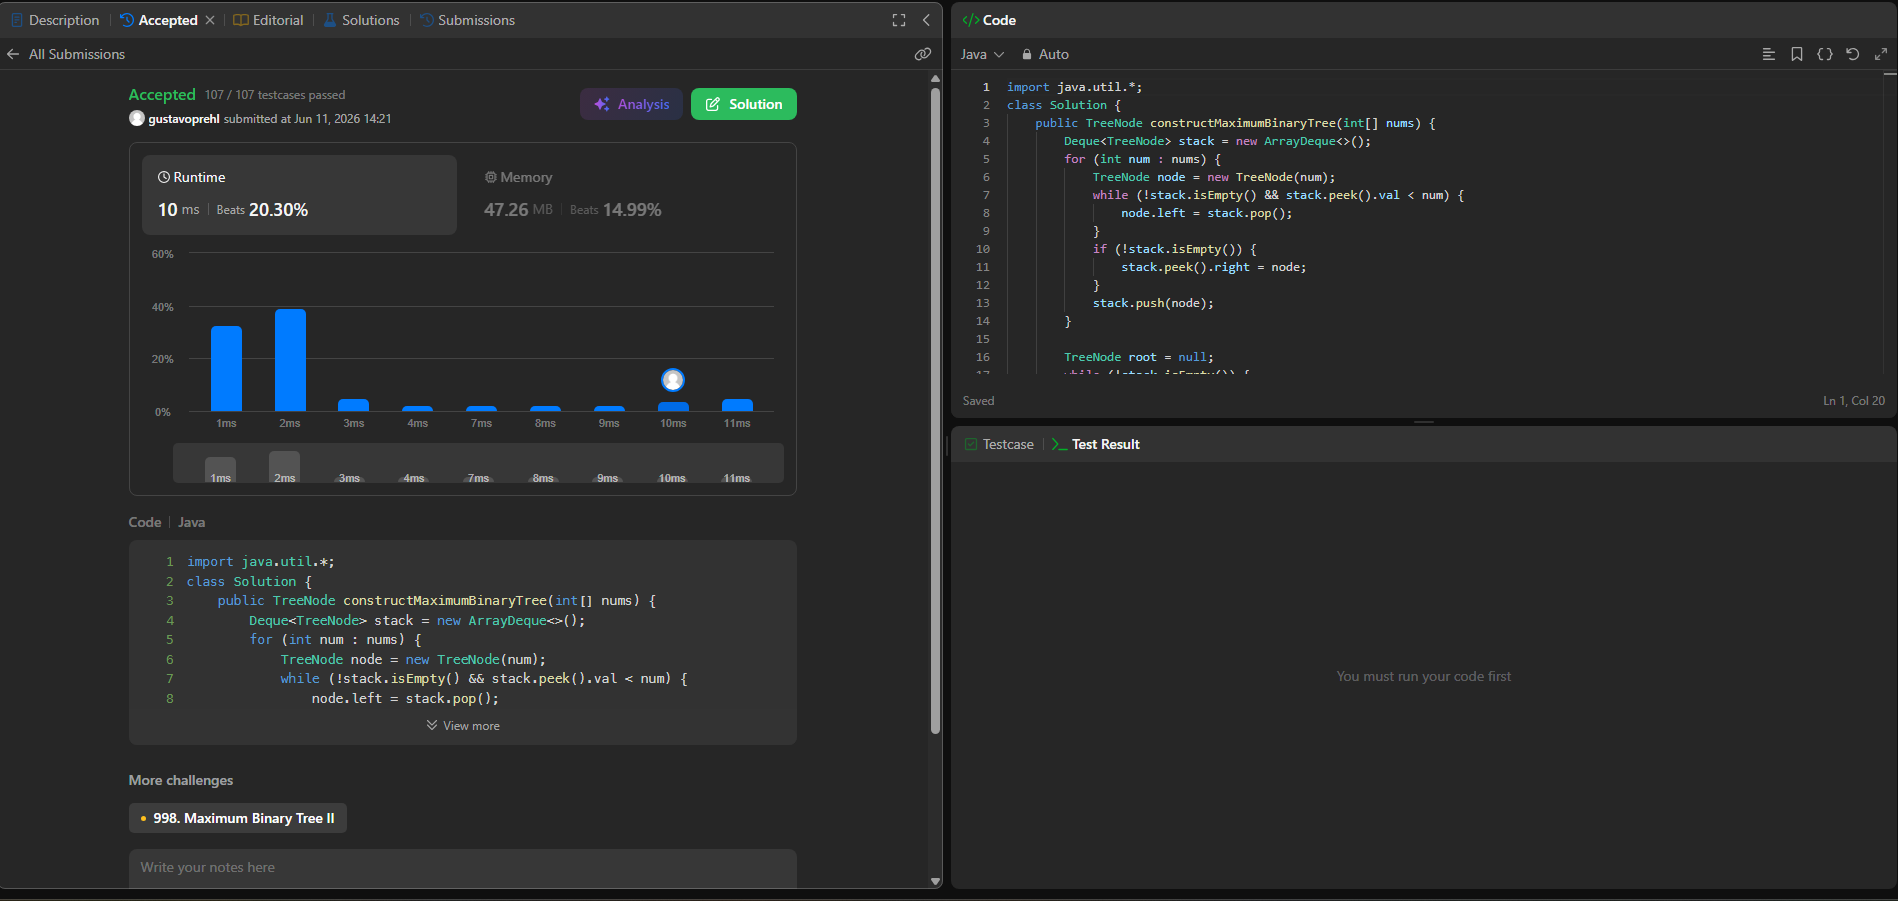
\includegraphics[width=0.85\textwidth]{Accepts/654_MaximumBinaryTree_Submit.png}\\
\end{center}

\subsection*{Justificativa}

\textbf{Estratégia:} pilha monotônica, construindo a árvore em uma única
passagem (em vez da abordagem ingênua $O(n^2)$ de buscar o máximo de cada
subarray recursivamente).

\textbf{Invariante da pilha:} a pilha mantém, do fundo para o topo, os nós
que ainda não encontraram, à sua direita, um valor maior que o seu --- ou
seja, candidatos a serem ``dominados'' por um número futuro. Os valores na
pilha são estritamente decrescentes do fundo para o topo, e cada nó é o
filho direito do nó imediatamente abaixo dele (formando a ``espinha
direita'' da árvore parcial construída até o momento).

\textbf{Relação com a definição recursiva do problema:} na árvore binária
máxima, o pai de um elemento \texttt{nums[i]} é o \textbf{menor} entre o
primeiro elemento maior à sua esquerda e o primeiro elemento maior à sua
direita (o ``dominador'' mais próximo). Ao processar \texttt{nums} da
esquerda para a direita:
\begin{itemize}
    \item Se o número atual é \textbf{maior} que o topo da pilha, ele é o
    primeiro elemento maior à direita de todos os nós removidos --- portanto,
    o número atual se torna ancestral deles. O último nó removido (o de
    maior valor entre os removidos, e portanto o mais próximo na hierarquia)
    vira o \textbf{filho esquerdo} do novo nó; os demais já estavam
    encadeados como filhos direitos uns dos outros, preservando a ordem
    relativa original.
    \item Se a pilha não ficou vazia após as remoções, o topo restante é o
    primeiro elemento maior à esquerda do número atual --- logo, o número
    atual se torna \textbf{filho direito} desse nó.
\end{itemize}

\textbf{Análise amortizada (custo $O(n)$):} cada elemento de \texttt{nums} é
empilhado exatamente uma vez e desempilhado no máximo uma vez durante toda a
execução. Pelo método agregado de análise amortizada, o número total de
operações de pilha (\emph{push} + \emph{pop}) ao longo das $n$ iterações é,
no máximo, $2n$, mesmo que o laço \texttt{while} interno execute múltiplas
vezes em iterações específicas.

\textbf{Complexidade:}
\begin{itemize}
    \item Tempo: $O(n)$ amortizado.
    \item Espaço: $O(n)$ para a pilha (no pior caso, array estritamente
    crescente).
\end{itemize}

\textbf{Tópico do curso:} a definição do problema --- o pai de cada elemento
é o menor entre os ``dominadores'' à esquerda e à direita --- corresponde a
uma formulação recursiva de divisão e conquista (\emph{Estratégia Gulosa e
Divisão e Conquista} [CLRS09, caps. 4 e 16]); a implementação com pilha
monotônica é a versão iterativa otimizada dessa recursão, cuja análise de
custo amortizado $O(n)$ se enquadra em \emph{Análise de Algoritmos
Iterativos} [CLRS09, caps. 1 e 2.2].
